%%% MEMOIR CLASS %%%
\documentclass[twoside,12pt,openright,final,english]{memoir}
% Memoir Divisions: \book, \part, \chapter, \section, \subsection
% Fine divisions:   \subsubsection, \paragraph \subparagraph.
%%% END MEMOIR CLASS %%%

\setlength{\parskip}{\baselineskip}%
\setlength{\parindent}{0pt}%

\usepackage{float}

\usepackage{graphicx}
% For full size print graphics
\graphicspath{{./images-original/}}

\makeindex
\makeglossary
\usepackage{color}
\usepackage[usenames,dvipsnames,svgnames,table]{xcolor}

%%% PAGE, STOCK, AND MARGIN SIZE %%%
% Lulu 7.44 x 9.68"   18.90 x 24.58cm
\setstocksize{24.58cm}{18.90cm} % { height }{ width }
\settrimmedsize{\stockheight}{\stockwidth}{*}

%\settypeblocksize{ height }{ width }{ ratio }
\settypeblocksize{19.0cm}{*}{*}

%\setlrmarginsandblock{ spine }{ edge }{ ratio }
% make the spine have more space than outer edge
\setlrmarginsandblock{*}{2.5cm}{1.2}

% \setulmargins{ upper }{ lower }{ ratio }
\setulmargins{2.0cm}{*}{*}

% \setheadfoot{ headheight }{ footskip }
\setheadfoot{12pt}{2cm}

\checkandfixthelayout[fixed]
%%% END PAGE, STOCK, AND MARGIN SIZE %%%

%%% INCLUDED FILES %%%
% select which chapters to render:
\newif\iftitle\titletrue
\newif\ifcopyright\copyrighttrue
\newif\ifintro\introtrue %true
\newif\ifgetting\gettingtrue %true
\newif\iffirst\firsttrue %true
\newif\iftuning\tuningtrue %true
\newif\iforganize\organizetrue %true
\newif\ifadvanced\advancedtrue %true
\newif\iftrouble\troubletrue %true
\newif\ifedge\edgetrue %true
\newif\ifsupport\supporttrue %true
\newif\ifcontact\contacttrue %true
\newif\ifcolophon\colophontrue %true

%% or just render everything:
\newif\ifrendereverything\rendereverythingfalse
\ifrendereverything \titletrue \copyrighttrue \introtrue \gettingtrue \firsttrue \tuningtrue \organizetrue \advancedtrue \troubletrue \edgetrue \supporttrue \contacttrue \colophontrue \fi
%%% END INCLUDED FILES %%%

\setcounter{secnumdepth}{3}
\setcounter{tocdepth}{3}

\usepackage[english]{babel}
\usepackage{ucs}

%%% PDFLATEX %%%
\usepackage{etex}

\usepackage[protrusion,expansion,spacing,kerning,babel,final]{microtype}
\usepackage[utf8x]{inputenc}

%%% PAGE STYLE %%%
\makepagestyle{jebstyle}
\pagestyle{jebstyle}
\makeevenhead{jebstyle}{}{\hspace{2em}\itshape\small\leftmark}{} % KLUDGE
\makeoddhead{jebstyle}{}{\scshape\small\rightmark}{}
\makeevenfoot{jebstyle}{}{\hspace{2em}\thepage}{} % KLUDGE
\makeoddfoot{jebstyle}{}{\thepage}{}
%%% END 

%%% jebinski CHAPTER STYLE %%%
\makechapterstyle{jebinski}{%
% Clear out the chapter name (e.g. capítulo)
  \renewcommand*{\printchaptername}{}
% Clear out the chapter number
  \renewcommand*{\printchapternum}{}
% Set chapter font
  \renewcommand*{\chaptitlefont}{\normalfont\large\scshape}
  \renewcommand*{\printchaptertitle}[1]{%
     \hrule\vskip\onelineskip \centering \chaptitlefont{##1}\par}
  \renewcommand*{\afterchaptertitle}{\vskip\onelineskip \hrule\vskip
     \afterchapskip}
}
%%% END jebinski CHAPTER STYLE %%%

%%% FORMATTING KLUDGES %%%
% fewer overfull lines compared with \fussy and fewer obvious
% large interword spaces than with \sloppy.
\midsloppy
% "fix" for Overfull \hbox
%\emergencystretch=8pt
\setlength{\emergencystretch}{3em}
% \tolerance is a paragraph parameter, probably ignored here
\tolerance=5000 % allow looser spacing 
%\tolerance=95000 % allow waaay looser spacing 
% 10000 almost prevents hyphenation. What's default?
\hyphenpenalty=500 % 500 seems reasonable
%the default \flushbottom
%\sloppypar
\setlength{\topskip}{1.6\topskip}
\checkandfixthelayout
%\sloppybottom
\raggedbottom
%%%%%%%% WIDOWS AND ORPHANS %%%%%%%%%%%
\widowpenalty=10000
\clubpenalty=10000
%%%%%%%% END WIDOWS AND ORPHANS %%%%%%%%%%%
%%% END FORMATTING KLUDGES %%%

%%% FOOTNOTES %%%
% no horizontal rule before footnotes:
\let\oldfootnoterule\footnoterule
\renewcommand*{\footnoterule}{}
% This indents the footnote, or it lines up too far to the
% left on the spanish side. The right page note should really
% move over more to the left
% KLUDGE
\setlength{\footmarkwidth}{3.5em}
%%% END FOOTNOTES %%%

%%% Fancy dings %%%
\usepackage{pifont}

%%% DEBUG %%%
%\showoutput
%\typeoutlayout
%\typeoutstandardlayout
%%% END DEBUG %%%


\usepackage[hidelinks]{hyperref}

%%% END OF PREAMBLE %%%

\begin{document}

%%% BEGIN FRONT MATTER %%%
\frontmatter

% Set page numbers to lowercase roman numerals, and reset the count to 1 (no *)
\pagenumbering{roman}

%%% TITLE PAGE %%%
% We want the title to be on the right hand page.
% If we pad a page, it gives us two with openright
\iftitle
{%!TEX root = Slic3r-Manual.tex
% clear the page style
\date {}
\thispagestyle{empty}
\begingroup
\centering 

\begin{center}
{\Huge \scshape Slic3r User Manual}

\end{center}

\vspace{40mm}

\begin{center}

\includegraphics[keepaspectratio=true,angle=0,height=0.25\textheight,width=0.25\textwidth]{slic3r.png}

\vspace{20mm}

{\large \itshape Gary Hodgson}

\vspace{20mm}

{\large \itshape Sponsored by }

\includegraphics[keepaspectratio=true,height=0.1\textheight]{lulzbot_logo.png}

\end{center}
\endgroup

}
\fi
%%% END TITLE PAGE

%%% COPYRIGHT PAGE %%%
\ifcopyright
{%!TEX root = Slic3r-Manual.tex
\clearpage\null\vfill
\begingroup
\thispagestyle{empty}
\footnotesize\raggedright
\setlength{\parskip}{0.5\baselineskip}

\textbf{Slic3r User Manual}

by Gary Hodgson (\href{http://garyhodgson.com}{garyhodgson.com})

Contributions by: Alessandro Ranellucci (\href{http://slic3r.org}{slic3r.org}), Jeff Moe (\href{http://lulzbot.com}{lulzbot.com})

Sponsored by LulzBot (\href{http://lulzbot.com}{lulzbot.com})

Copyright \copyright\ \the\year\ Aleph Objects, Inc.\par
Permission is granted to copy, distribute and\slash or modify
this document under the terms of the
Creative Commons Attribution-ShareAlike 3.0 Unported license
(CC BY-SA 3.0).

Published by Free Software Folks

\hfill\texttt{\the\year\ifnum\month<10 0\fi\the\month
                \ifnum\day  <10 0\fi\the\day}
\endgroup
\pagebreak{}
}
\fi
%%% END COPYRIGHT PAGE %%%


%%% TABLE OF CONTENTS ToC %%%
\maxtocdepth{section}
% Dots
% space between dots
\renewcommand{\cftchapterdotsep}{15}
% dot symbol (default is period)
\renewcommand{\cftdot}{\textperiodcentered}	% centered period
% Set space between each entry in ToC
\setlength{\cftbeforechapterskip}{5pt}  % 5pt % 3pt
\tableofcontents*
%%% END TABLE OF CONTENTS ToC %%%

%%% LIST OF FIGURES %%%
%\addtodef{\listoffigures}{\clearpage\pagestyle{lof}}{}
% Fit all of List of Figures on one page
\renewcommand*{\lofheadstart}{\vspace{1cm}}
\clearpage
\listoffigures*
%%% END LIST OF FIGURES %%%

%%% CHAPTER STYLE %%%
\chapterstyle{jebinski} % defined in preamble
\def\topblockvspace{0.11}

%%% END FRONTMATTER %%%
%%% BEGIN MAINMATTER %%%
\mainmatter*

% Set page numbering to arabic, but don't reset numbering (*)
\pagenumbering*{arabic}

%%% Introduction %%%
\ifgetting
\chapter{\emph{Introduction}}
\thispagestyle{empty}
\markboth{Introduction}{Slic3r User Manual}
{%!TEX root = Slic3r-Manual.tex
\section{Overview}
Slic3r is a tool which translates digital 3D models into instructions that are understood by a 3D printer.  It slices the model into horizontal layers and generates suitable paths to fill them.

Slic3r is already bundled with the many of the most well-known host software packages: Pronterface, Repetier-Host, ReplicatorG, and can be used as a standalone program.

This manual will provide guidance on how to install, configure and utilise Slic3r in order to produce excellent prints.


\section{Goals \& Philosophy}
Slic3r is an original project started in 2011 by Alessandro Ranellucci (aka. Sound), who used his considerable knowledge of the Perl language to create a fast and easy to use application.  Readability and maintainability of the code are among the design goals.

The program is under constant refinement, from Alessandro and the other contributors to the project, with new features and bug fixes being released on a regular basis.


\section{Donating}
Slic3r started as a one-man job, developed solely by Alessandro in his spare time, and as a freelance developer this has a direct cost for him.  By generously releasing Slic3r to the public as open source software, under the GPL license, he has enabled many to benefit from his work.

The opportunity to say thank you via a donation exists.  More details can be found at: \texttt{http://slic3r.org/donations}.}
\fi
%%% END Introduction %%%

%%% GETTING SLIC3R %%%
\ifgetting
\chapter{\emph{Getting Slic3r}}
\thispagestyle{empty}
\markboth{Getting Slic3r}{Slic3r User Manual}
{%!TEX root = Slic3r-Manual.tex
\index{download}
\index{binaries}
\index{Source Code}
\index{GitHub}
\index{license}

\fbox{
	\parbox{\linewidth}{
		Slic3r is Free Software, and is licensed under the GNU Affero General Public License, version 3.
	}
}	

\section{Downloading}

\subsection{Slic3r} % (fold)
\label{sub:slic3r}
Slic3r can be downloaded directly from: \url{http://slic3r.org/download}.

Pre-compiled packages are available for Windows, Mac OS X and Linux.  Windows and Linux users can choose between 32 and 64 bit versions to match their system.
% subsection slic3r (end)

\subsection{Manual} % (fold)
\label{sub:manual}

The latest version of this document, with {\LaTeX} source code, can be found at: \url{https://github.com/alexrj/Slic3r-Manual}

% subsection manual (end)

\subsection{Source} % (fold)
\label{sub:source}

The source code is available via GitHub: \url{https://github.com/alexrj/Slic3r}. For more details on building from source see §\ref{sec:building_from_source} below.

% subsection source (end)

\section{Installing}

\subsection{Windows}

Unzip the downloaded zip file to a folder of your choosing, there is no installer script. The resulting folder contains two executables:
\begin{itemize}
\item \texttt{slic3r.exe} - starts the GUI version.
\item \texttt{slic3r-console.exe} - can be used from the command line.
\end{itemize}

The zip file may then be deleted.

\subsection{Mac OS X}

Double-click the downloaded dmg file, an instance of Finder should open together with an icon of the Slic3r program.  Navigate to the Applications directory and drag and drop the Slic3r icon into it.
The dmg file may then be deleted.

\subsection{Linux}

Extract the archive to a folder of your choosing.
Either:
\begin{itemize}
\item Start Slic3r directly by running the Slic3r executable, found in the bin directory, or
\item Install Slic3r by running the do-install executable, also found in the bin folder.
\end{itemize}
The archive file may then be deleted.



\section{Building from source} % (fold)
\label{sec:building_from_source}

For those wishing to live on the cutting edge, Slic3r can be compiled from the latest source files found on GitHub\footnote{\url{https://github.com/alexrj/Slic3r}}.

Up-to-date instructions for compiling and running from source can be found on the Slic3r wiki.

\begin{itemize}
    \item \textbf{GNU Linux} \par\url{https://github.com/alexrj/Slic3r/wiki/Running-Slic3r-from-git-on-GNU-Linux}
    \item \textbf{OS X} \par\url{https://github.com/alexrj/Slic3r/wiki/Running-Slic3r-from-git-on-OS-X}
    \item \textbf{Windows} \par\url{https://github.com/alexrj/Slic3r/wiki/Running-Slic3r-from-git-on-Windows}

\end{itemize}
}
\fi
%%% END GETTING SLIC3R %%%

%%% FIRST PRINT %%%
\ifgetting
\chapter{\emph{First Print}}
\thispagestyle{empty}
\markboth{First Print}{Slic3r User Manual}
{%!TEX root = Slic3r-Manual.tex

\section{First Print} % (fold)
\label{sec:first_print}

At this stage Slic3r has been configured and a model has been acquired, sliced and made ready for print.  Now would be the time to fire up the printer and try it out.

A variety of host software is available to send the G-code to the printer.  Amongst the open-source solutions are: Printrun\footnote{https://github.com/kliment/Printrun}, Repetier\footnote{http://www.repetier.com/} and Repsnapper\footnote{https://github.com/timschmidt/repsnapper}.

The following sections will cover the options available in expert mode, and look at advanced printing techniques, including special cases and troubleshooting.

% section first_print (end)}
\fi
%%% END FIRST PRINT %%%

%%% EXPERT MODE %%%
\ifadvanced
\chapter{\emph{Expert Mode}}
\thispagestyle{empty}
\markboth{Expert Mode}{Slic3r User Manual}
{%!TEX root = Slic3r-Manual.tex


%!TEX root = Slic3r-Manual.tex

\section{Speed} % (fold)
\label{sec:speed}
\index{speed}

Once the printer is reliably producing good quality prints it may be desirable to increase the speed.  Doing this provides several benefits, the most obvious of which is that the results are produced quicker, but also faster print times can be utilised in producing more layers, i.e. lower layer height, thus improving perceived print quality.  An additional benefit is that a faster travel movement, between extrusions, can reduce the effects of oozing.

The best approach is to increment the various speed parameters in small steps and observe the effect each change has on print quality.  Travel speed is a safe starting point, and it is not unrealistic to attain speeds of up to 250mm/s (if your printer can handle it).  Adjusting the speed of perimeters, infill is available in simple mode, and the general rule is to have the perimeter go a little slower than the infill in order to reduce possible blemishes on the surface (infill can be faster because slight gaps will not matter as much).

Expert mode offers more parameters to fine tune printer speeds.  Differentiation between external, small and other perimeters, infill locations, and bridges and gaps are available, as well as the ability to slow down for the first layer.

\begin{figure}[H]
\centering
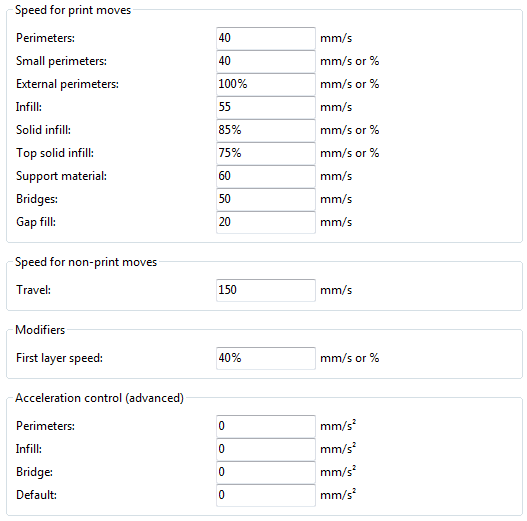
\includegraphics[keepaspectratio=true,width=1\textwidth]{expertmode/speed_advanced_settings.png}
\caption{Expert mode speed options.}
\label{fig:speed_advanced_settings}
\end{figure}

Where indicated a value can be given in percentage.  This is in relation to the preceding value, e.g. 50\% solid infill would be half of the value defined for infill.

A few general guidelines for each option:
\begin{itemize}
	\item \texttt{Perimeters}  - In expert mode this parameter can be increased slightly as the \texttt{External perimeters} option can be used to ensure blemish free external faces.
	\item \texttt{Small perimeters}  - Meant for holes, islands and fine details, a slower speed here is recommended.
	\item \texttt{External perimeters}  - A slightly slower value may ensure cleaner surfaces.
	\item \texttt{Infill}  - As fast as you can without compromising the integrity of the fill structure.  Faster extrusions can break and result in weak spots.
	\item \texttt{Solid infill}  - The bottom of the model, and any additional solid layers is usually slightly slower than infill but faster than perimeters.
	\item \texttt{Top solid infill}  - Allow time for the extrusion to cleanly cover the previous top layers and result in a tidy top surface.  the last few layers should have bridged the infill structure nicely, preparing the way for a neat finish.
	\item \texttt{Support material}  - Generally support structures are quick and dirty, and so long as the base is adequately supported they can be built as quickly as they can.
	\item \texttt{Bridges}  - Having the extrusion span distances depends on the material and cooling.  Going too slow will result in sagging, too fast will result in broken strands.  Experimentation is the key here, but generally bridging runs slower than perimeters.
	\item \texttt{Gap fill}  - Filling in small gaps results in the extruder quickly oscillating and the resulting shaking and resonance could have a detrimental affect on the printer.  A smaller value here can guard against this.  A setting of zero disables gap filling completely.
	\item \texttt{Travel}  - As fast as your printer will allow in order to minimise ooze.
	\item \texttt{First layer speed}  - As mentioned in section \ref{sec:the_important_first_layer}, the first layer is important to lay down correctly, and a slower pace helps enormously.  Setting a value of 50\%, or even less, can really help.
\end{itemize}

\texttt{Acceleration control} is an advanced setting allowing acceleration settings for perimeters, infill, bridge, as well as a default setting, to be made.  Deciding which values to set depends on the capabilities of the machine.  Any settings within the firmware may be a good starting point.

Take into account any restrictions enforced by the firmware as many have settings for the maximum safe speed of each axis.

% section speed (end)

\newpage

%!TEX root = Slic3r-Manual.tex

\section{Infill Patterns and Density} % (fold)
\label{sec:infill_patterns_and_density}
\index{infill}

There are several considerations when choosing an infill pattern: object strength, time and material, personal preference.  It can be inferred that a more complex pattern will require more moves, and hence take more time and material.  

\begin{figure}[H]
\centering
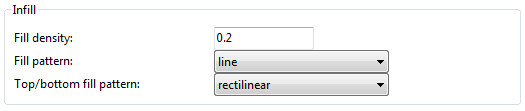
\includegraphics[keepaspectratio=true,width=1.0\textwidth]{expertmode/infill_pattern_settings.png}
\caption{Infill pattern settings.}
\label{fig:infill_pattern_settings}
\end{figure}

Slic3r offers several infill patterns, four regular, and three more exotic flavours.  The numbers given in brackets below each figure are a rough estimate of material used and time taken for a simple 20mm cube model\footnote{Taken from http://gcode.ws}.  Note that this is only indicative, as model complexity and other factors will affect time and material.

\begin{figure}[H]
\centering
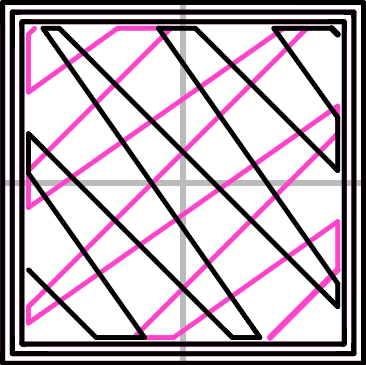
\includegraphics[keepaspectratio=true,width=0.2\textwidth]{expertmode/infill_line.png}
\caption{Infill pattern: Line (344.51mm / 5m:20s)}
\label{fig:infill_line}
\end{figure}

\begin{figure}[H]
\centering
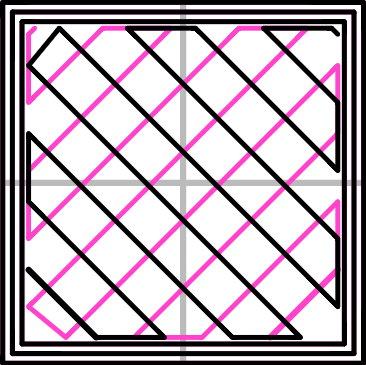
\includegraphics[keepaspectratio=true,width=0.2\textwidth]{expertmode/infill_rectilinear.png}
\caption{Infill pattern: Rectilinear (350.57mm / 5m:23s)}
\label{fig:infill_rectilinear}
\end{figure}

\begin{figure}[H]
\centering
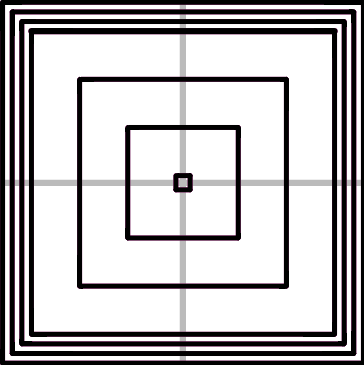
\includegraphics[keepaspectratio=true,width=0.2\textwidth]{expertmode/infill_concentric.png}
\caption{Infill pattern: Concentric (351.80mm / 5m:30s)}
\label{fig:infill_concentric}
\end{figure}

\begin{figure}[H]
\centering
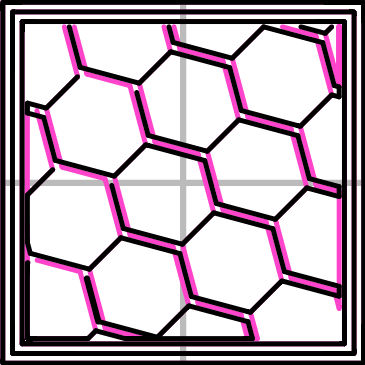
\includegraphics[keepaspectratio=true,width=0.2\textwidth]{expertmode/infill_honeycomb.png}
\caption{Infill pattern: Honeycomb (362.73mm / 5m:39s)}
\label{fig:infill_honeycomb}
\end{figure}

\begin{figure}[H]
\centering
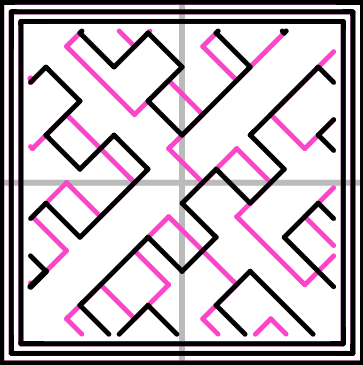
\includegraphics[keepaspectratio=true,width=0.2\textwidth]{expertmode/infill_hilbertcurve.png}
\caption{Infill pattern: Hilbert Curve (332.82mm / 5m:28s)}
\label{fig:infill_hilbertcurve}
\end{figure}

\begin{figure}[H]
\centering
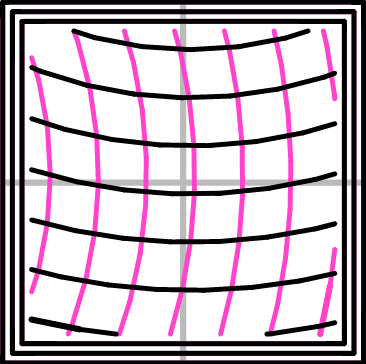
\includegraphics[keepaspectratio=true,width=0.2\textwidth]{expertmode/infill_archimedeanchords.png}
\caption{Infill pattern: Archimedean Chords (333.66mm / 5m:27s)}
\label{fig:infill_archimedeanchords}
\end{figure}

\begin{figure}[H]
\centering
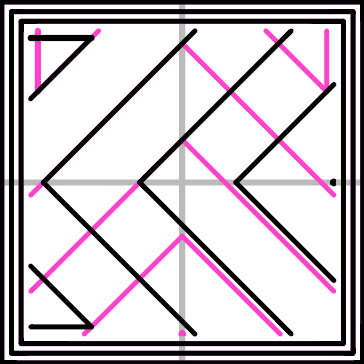
\includegraphics[keepaspectratio=true,width=0.2\textwidth]{expertmode/infill_octagramspiral.png}
\caption{Infill pattern: Octagram Spiral (318.63mm / 5m:15s)}
\label{fig:infill_octagramspiral}
\end{figure}


Certain model types are more suited for a particular pattern, for example organic versus mechanical types.  Figure \ref{fig:complex_object_infill_comparison} shows how a honeycomb fill may suit this mechanical part better because each hexagon bonds with the same underlying pattern each layer, forming a strong vertical structure.

\begin{figure}[H]
\centering
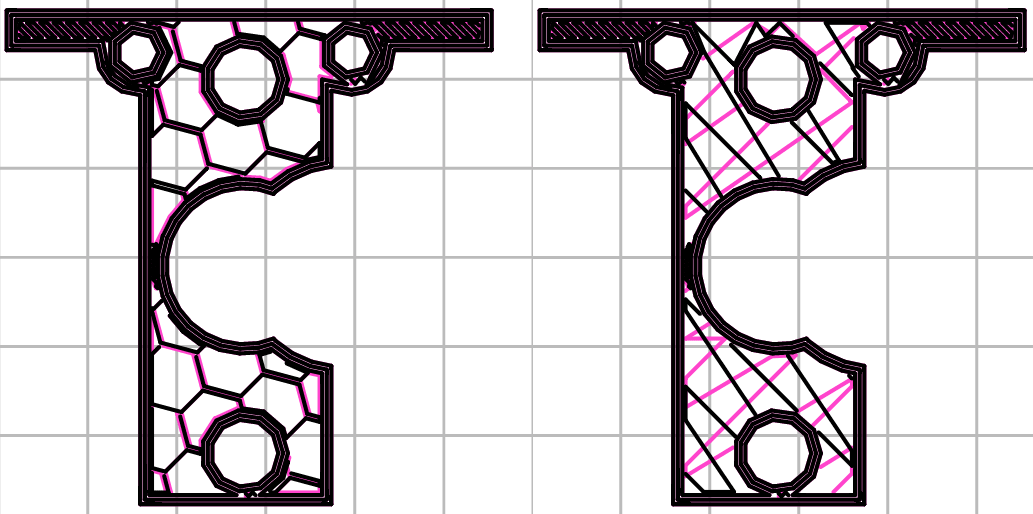
\includegraphics[keepaspectratio=true,width=0.75\textwidth]{expertmode/complex_object_infill_comparison.png}
\caption{Infill pattern comparison in a complex object. Left to Right: honeycomb, line}
\label{fig:complex_object_infill_comparison}
\end{figure}

Most models require only a low density infill, as providing more than, say, 50\% will produce a very tightly packed model which uses more material than required.  For this reason a common range of patterns is between 10\% and 30\%, however the requirements of the model will determine which density is best.  Figure \ref{fig:infill_pattern_densities} shows how the patterns change as the density increases.
\begin{figure}[H]
\centering
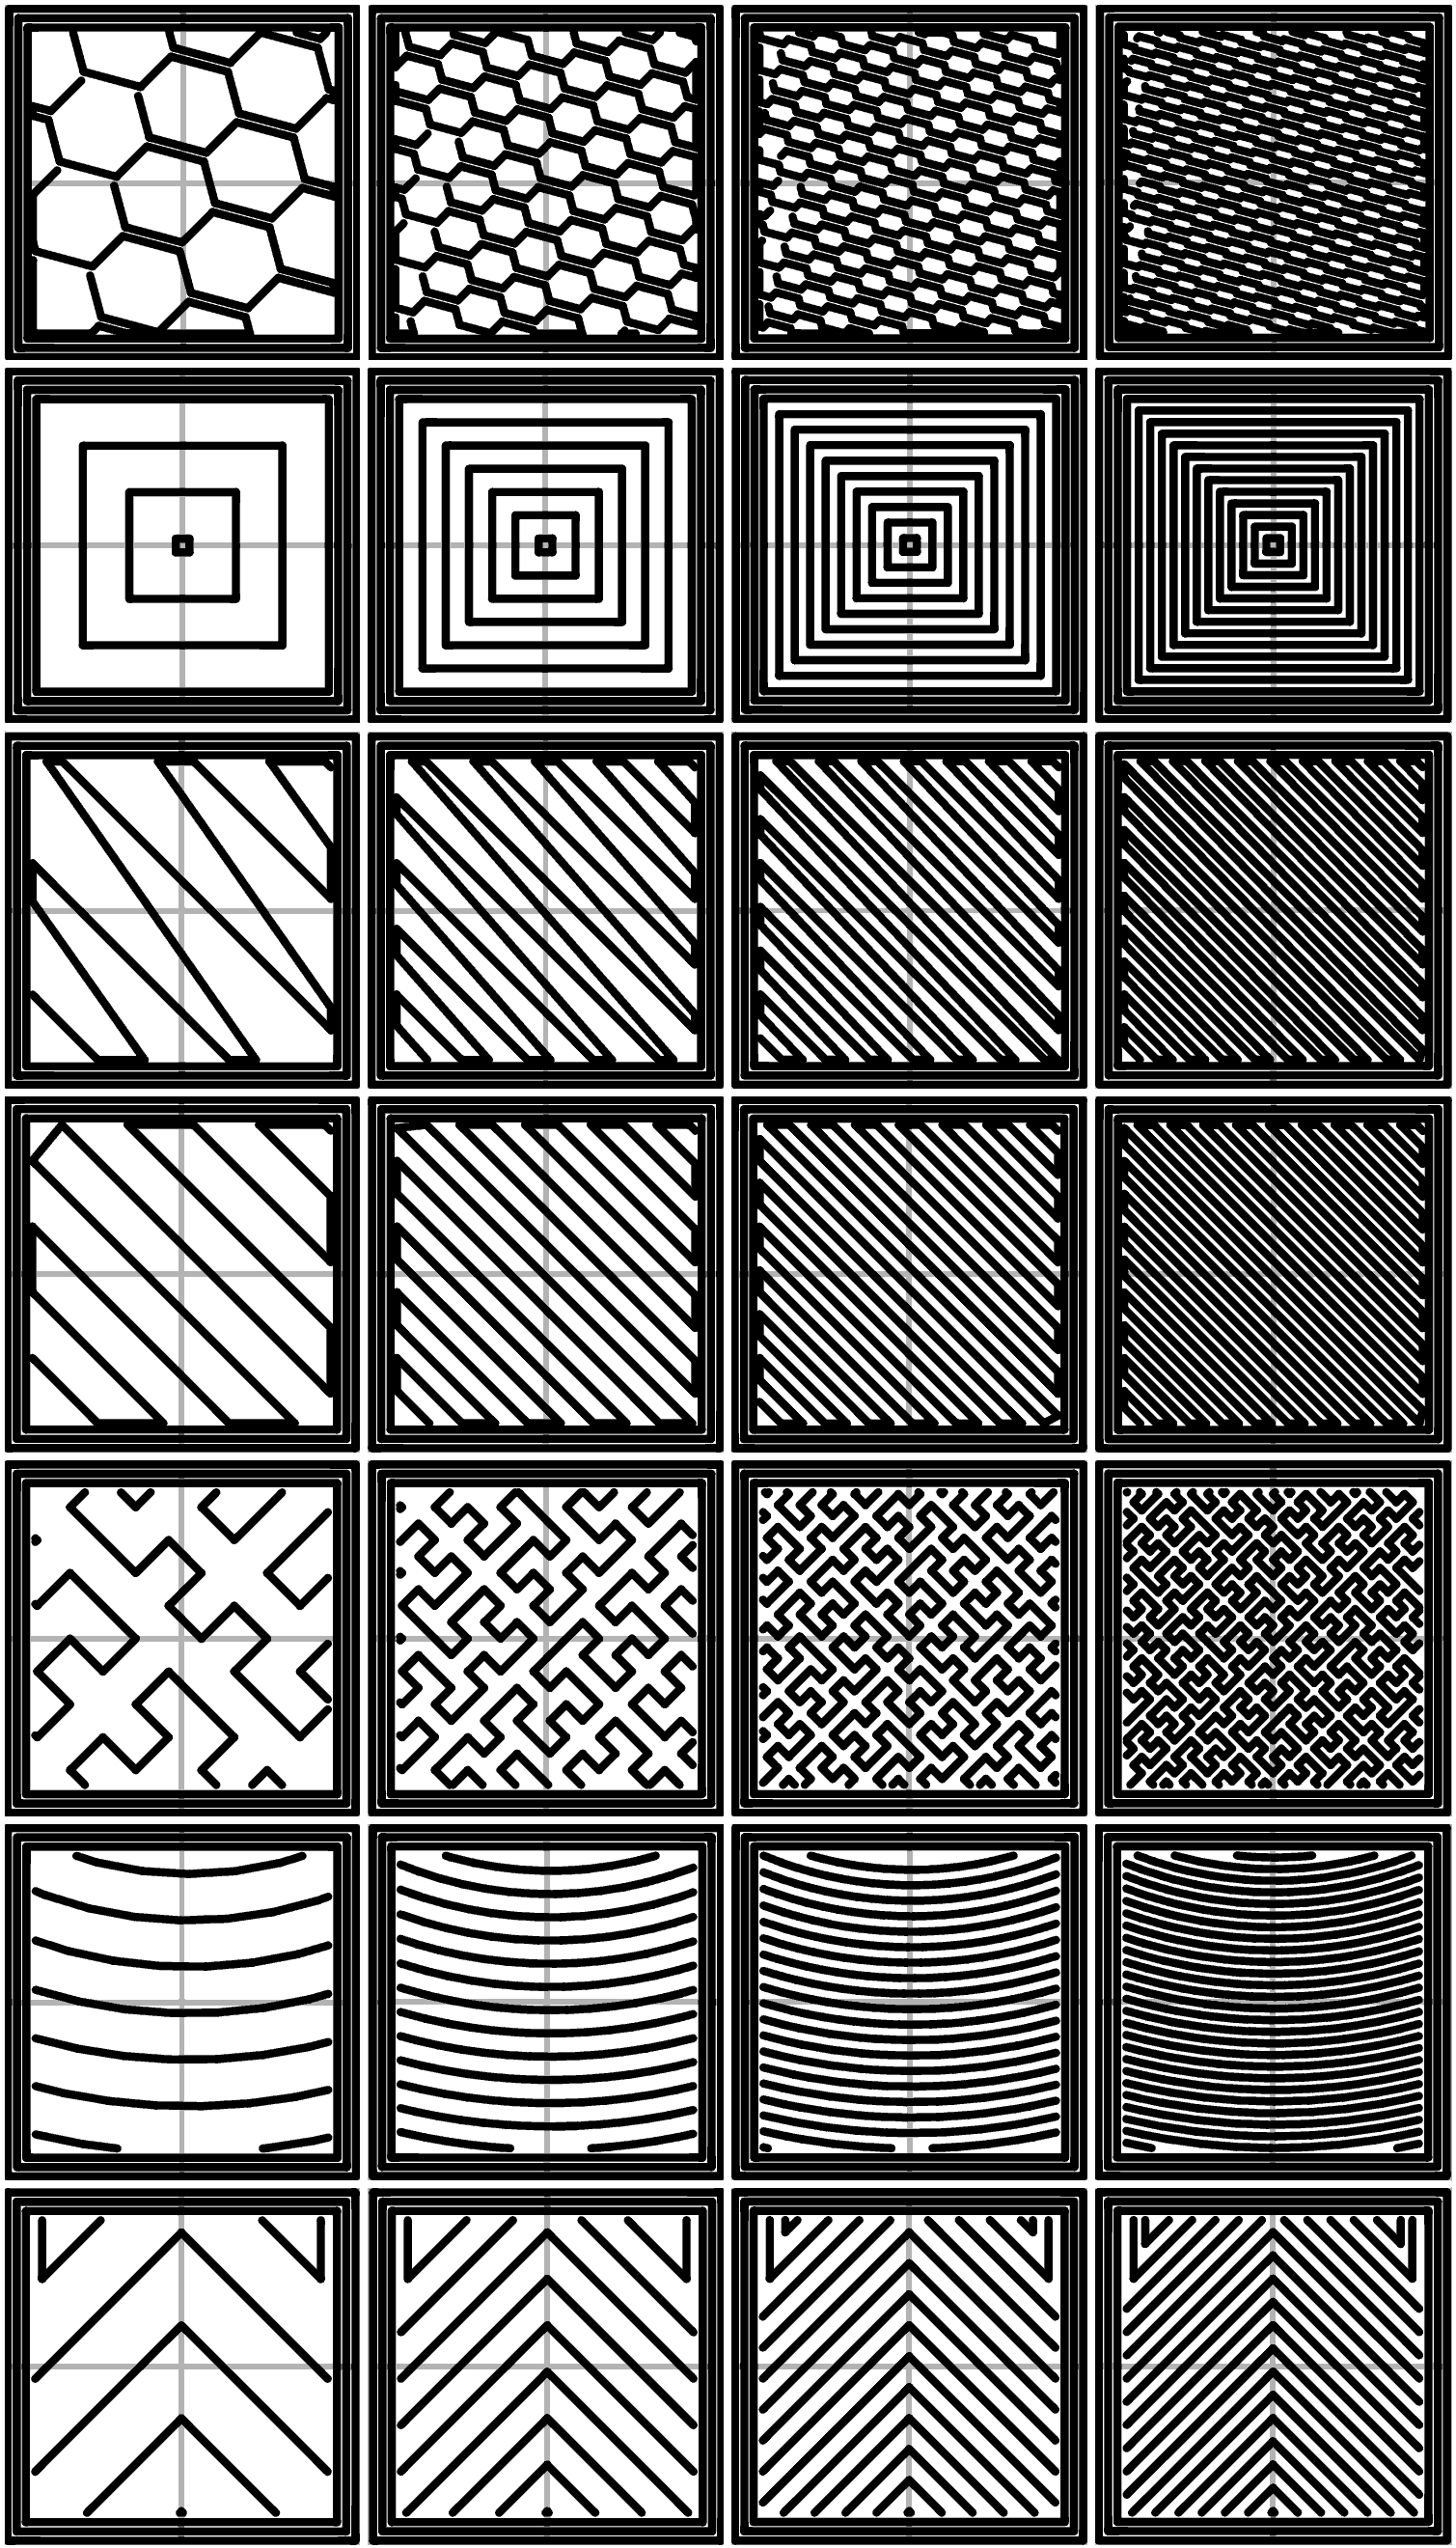
\includegraphics[keepaspectratio=true,width=0.7\textwidth]{expertmode/infills.png}
\caption{Infill patterns at varying densities. Left to Right: 20\%,40\%,60\%,80\%. Top to Bottom: Honeycomb, Concentric, Line, Rectilinear, Hilbert Curve, Archimedean Chords, Octagram Spiral}
\label{fig:infill_pattern_densities}
\end{figure}

% section infill_patterns_and_density (end)

\newpage

%!TEX root = Slic3r-Manual.tex


\section{Infill Optimization} % (fold)
\label{sec:infill_optimization}

Slic3r contains several advanced infill settings which can help produce better extrusions.

\begin{figure}[H]
\centering
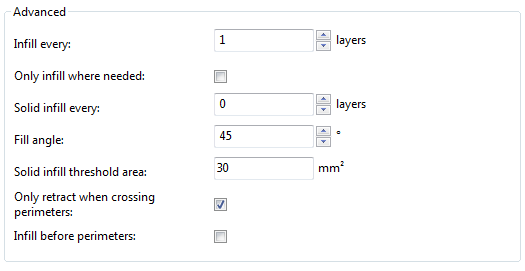
\includegraphics[keepaspectratio=true,width=1.0\textwidth]{expertmode/infill_advanced_settings.png}
\caption{Infill advanced settings.}
\label{fig:infill_settings}
\end{figure}

\begin{itemize}
    \item \texttt{Infill every \textit{n} layers} - Will produce sparse vertical infill by skipping a set number of layers. This can be used to speed up print times where the missing infill is acceptable.
    \item \texttt{Only infill where needed} - Slic3r will analyse the model and choose where infill is required in order to support internal ceilings and overhangs.  Useful for reducing time and materials.
    \item \texttt{Solid infill every \textit{n} layers} - Forces a solid fill pattern on the specified layers.  Zero will disable this option.
    \item \texttt{Fill angle} - By default the infill pattern runs at 45° to the model to provide the best adhesion to wall structures.  Infill extrusions that run adjacent to perimeters are liable to de-laminate under stress.  Some models may benefit from rotating the fill angle to ensure the optimal direction of the extrusion.
    \item \texttt{Solid infill threshold area} - Small areas within the model are usually best off being filled completely to provide structural integrity.  This will however take more time and material, and can result in parts being unnecessarily solid.  Adjust this option to balance these needs.
    \item \texttt{Only retract when crossing perimeters} - Retracting, to prevent ooze, is unnecessary if the extruder remains within the boundaries of the model.  Care should be taken if the print material oozes excessively, as not retracting may result in enough material loss to affect the quality of the subsequent extrusion.  However, most modern printers and materials rarely suffer from such extreme ooze problems.
    \item \texttt{Infill before perimeters} - Reverses the order in which the layer is printed. Usually the perimeter is laid down initially, followed by the infill, and this is usually the preferable as the perimeter acts as a wall containing the infill.
\end{itemize}


% section infill_optimization (end)

\newpage

%!TEX root = Slic3r-Manual.tex

\section{Fighting Ooze} % (fold)
\label{sec:fighting_ooze}

Unless the material being extruded has a very high viscosity it will ooze from the nozzle in between extrusions.  There are several settings in Slic3r to which can help to remedy this.

The retraction settings, found in the \texttt{Printer} tab, tell the printer to pull back the filament between extrusion moves.  This can alleviate the pressure in the nozzle, thus reducing ooze.  After the subsequent travel move the retraction is reversed to prepare the extruder for the next extrusion.

\begin{figure}[H]
\centering
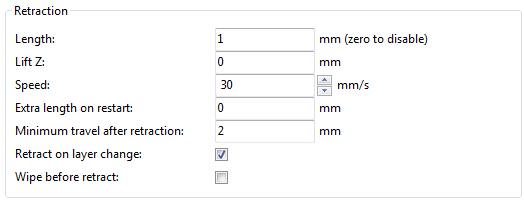
\includegraphics[keepaspectratio=true,width=1.0\textwidth]{expertmode/retraction_settings.png}
\caption{Retraction settings.}
\label{fig:retraction_settings}
\end{figure}

\begin{itemize}
    \item \texttt{Length} - The number of millimeters to retract.  Note that the measurement is taken from the raw filament entering the extruder.  A value of between 1 and 2mm is usually recommended. Bowden extruders may need up to 4 or 5mm due to the hysteresis introduced by the tube.
    \item \texttt{Lift Z} - Raises the entire extruder on the Z axis by that many millimeters during each travel.  This can be useful to ensure the nozzle will not catch on any already laid filament, however it is usually not necessary and will slow the print speed.  A value of 0.1mm is usually sufficient.
    \item \texttt{Speed} - The speed at which the extruder motor will pull back the filament.  The value should be set to as quick as the extruder can handle without skipping steps, and it is worth experimenting with this value to find the quickest retraction possible.
    \item \texttt{Extra length on restart} -  Adds an extra length of filament after the retraction is compensated after the travel move. This setting is rarely used, however should the print show signs of not having enough material after travel moves then it may be useful to add a small amount of additional material.
    \item \texttt{Minimum travel after retraction} - Triggering a retraction after very short moves is usually unnecessary as the amount of ooze is usually insignificant and it slows down the print times.  Set the number of millimeters minimum distance the nozzle must move before considering a retraction.  If the printer handles ooze well this can be increased to 5 or 6mm.
    \item \texttt{Retract on layer change} - Movement along the Z axis must also be considered when dealing with oozing, otherwise blobs may occur.  It is recommended to leave this setting on.
    \item \texttt{Wipe before retract} - Moves the nozzle whilst retracting so as to reduce the chances of a blob forming.
\end{itemize}


Additionally there are several settings in the \texttt{Print} tab which can help control oozing.

\begin{itemize}
    \item \texttt{Only retract when crossing perimeters} (Infill) - Tells Slic3r to only retract if the nozzle will cross the threshold of the current island being extruded.  Slight ooze within the walls of a part are not seen and can usually be accepted.
    \item \texttt{Avoid crossing perimeters} (Layers and perimeters - Advanced) - Will force the nozzle to follow perimeters as much as possible to minimise the number of times it must cross them when moving around, and between, islands.  This has a negative impact on both G-code generation and print times.
    \item \texttt{Randomize starting points} (Layers and perimeters - Vertical shells) - As the extruder moves up to the start of the next layer any ooze can result in blobs.  If the same start point is used for every layer then a seam can form the length of the object.  This setting will move the start point to a difference location for each layer.    
\end{itemize}
% section fighting_ooze (end)

\newpage

%!TEX root = Slic3r-Manual.tex

\section{Skirt} % (fold)
\label{sec:skirt}

The \texttt{Skirt} setting adds an extrusion a short distance away from the perimiter of the object.  This can ensure that the material is flowing smoothly from the extruder before it starts on the model proper.

\begin{figure}[H]
\centering
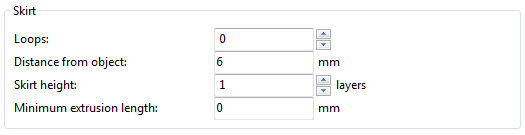
\includegraphics[keepaspectratio=true,width=1.0\textwidth]{expertmode/skirt_settings.png}
\caption{Skirt settings.}
\label{fig:skirt_settings}
\end{figure}

\begin{itemize}
    \item \texttt{Loops} - How many circuits should be completed before starting on the model.  One loop is usually sufficient.
    \item \texttt{Distance from object} - The millimeters between the object and the skirt.  The default of 6mm is usually sufficient.
    \item \texttt{Skirt height} - The number of layers to lay down a skirt for.  For ensuring the material is flowing smoothly, one layer is sufficient, however the skirt function can also be used to build walls around the object in case it should be protected from draughts.
    \item \texttt{Minimum extrusion length} - Dictates a minimum number of millimeters that the skirt should be, should the loop around the object not be enough.
\end{itemize}

% section skirt (end)

\newpage

%!TEX root = Slic3r-Manual.tex

\section{Cooling} % (fold)
\label{sec:cooling}
\index{cooling}
\index{temperature}

Temperature plays a key part in determining print quality.  Too hot and the material deforms, too cool and layer adhesion may be problematic.  Applying cooling will allow the freshly deposited material to solidify enough to provide a good base for the next layer, helping with overhangs, small details and bridges.

There are two main techniques for cooling: adding a fan and slowing down the print speed.  Slic3r may choose to use both techniques, using a fan first, and then slowing down the print if the layer time is too fast.

\begin{figure}[H]
\centering
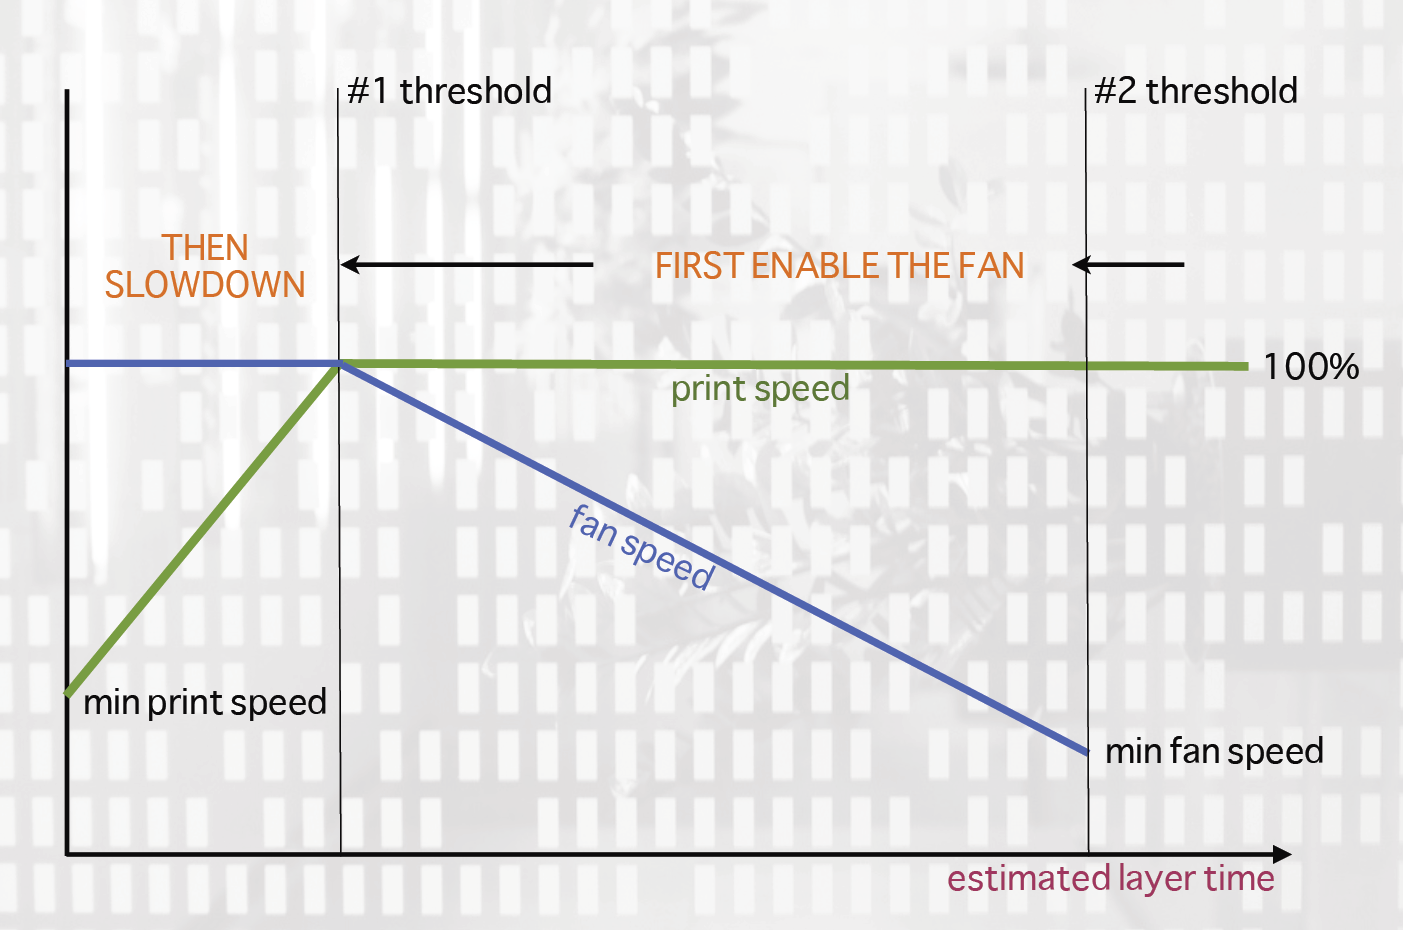
\includegraphics[keepaspectratio=true,width=1\textwidth]{expertmode/cooling_chart.png}
\caption{Cooling strategy.}
\label{fig:cooling_chart}
\end{figure}

Figure \ref{fig:cooling_chart} shows the strategy adopted by Slic3r.  Reading from right to left, when the minimum fan threshold (\#2) is reached the fan is turned on.  This increases in intensity as the layer time decreases.  The print speed remains constant until the estimated print time drops below a certain threshold (\#1), this is when the print speed is reduced until it reaches it's minimum value.

\subsection{Fans} % (fold)
\label{sub:fans}
\index{cooling!fans}
Most electronics and firmware allow the addition of a fan via a spare connector.  These can then be instructed with G-code, from Slic3r, to turn on or off as the model requires, and to rotate at different speeds.

Care should be taken with the positioning of the fan so that it does not cool any heated bed more than necessary.  It should also not cool the heater block of the hot-end so as not to force it to do more work and waste energy.  The air movement should aim for the nozzle tip, flowing over the freshly extruded material.

A duct may help in guiding the flow correctly, and there are several designs available online, for a wide variety of printers.

% subsection fans (end)

\subsection{Slowing Down} % (fold)
\label{sub:slowing_down}
\index{cooling!slowing down}
Slic3r can tell the printer to slow down if the estimated layer time is above a certain threshold.

Care must be taken as the intended effect could be mitigated by the nozzle not moving far enough away from the fresh extrusion, a problem with small, detailed layers.  For this reason it is usually recommended to use a fan where possible.
% subsection slowing_down (end)

\subsection{Configuring} % (fold)
\label{sub:configuring_cooling}

In simple mode Slic3r will attempt to choose the optimal settings for both fans and speed.  Expert mode gives more granular options.

\begin{figure}[H]
\centering
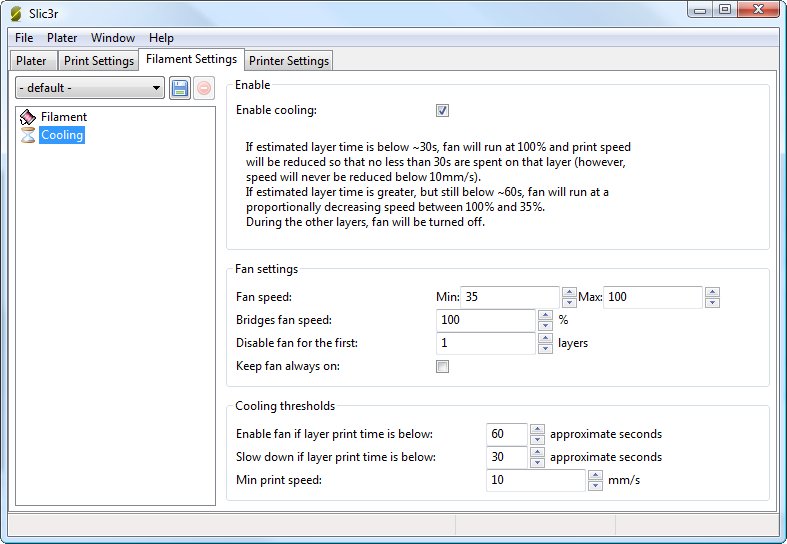
\includegraphics[keepaspectratio=true,width=1\textwidth]{expertmode/cooling_advanced_settings.png}
\caption{Cooling advanced settings.}
\label{fig:cooling_advanced_settings}
\end{figure}

\begin{itemize}
    \index{Filament Settings!Cooling!Fan speed}
	\item \texttt{Fan speed}  - Determines the minimum and maximum speeds - useful for fans that run too fast by default.
    \index{Filament Settings!Cooling!Bridges fan speed}
	\item \texttt{Bridges fan speed}  - As the material stretches over wide gaps, it makes sense to try and cool it as much as possible, therefore a full fan speed is recommended.
    \index{Filament Settings!Cooling!Disable fan for first n layers}
	\item \texttt{Disable fan for first \textit{n} layers}  - Section \ref{sec:the_important_first_layer} detailed how important the first layer is, and so it makes sense not to apply the fan until sure the print is securely attached to the bed.  Keeping the fan turned off for the first two or three layers is a good idea.
    \index{Filament Settings!Cooling!Keep fan always on}
	\item \texttt{Keep fan always on}  - Overrides any other choices and has the fan run continuously, at least at the minimum speed setting.  This can be useful when printing with PLA, but is not recommended for ABS.
\end{itemize}

\begin{itemize}
    \index{Filament Settings!Cooling!Enable fan if print time is below t seconds}
	\item \texttt{Enable fan if print time is below \textit{t} seconds}  - Triggers the fan if the layer will be completed within the given number of seconds.
    \index{Filament Settings!Cooling!Slow down if layer print time is below t seconds}
	\item \texttt{Slow down if layer print time is below \textit{t} seconds}  - Slows down the print if the layer will be completed within the given number of seconds.
    \index{Filament Settings!Cooling!Min print speed}
	\item \texttt{Min print speed}  - A lower limit on how slowly a layer can be printed.
\end{itemize}


% subsection configuring_cooling (end)

% section cooling (end)

\newpage

%!TEX root = Slic3r-Manual.tex
\section{Support Material} % (fold)
\label{sec:support}
\index{support material}

Generally, most 3D models will print with overhanging parts by up to a certain degree.  The angle is determined by several factors, most notably layer height and extrusion width, and is usually around 45°.  For models with larger overhangs a support structure may have to be printed below it.  This incurs the use of more material, longer print times, and post printing clean-up.

\begin{figure}[H]
\centering
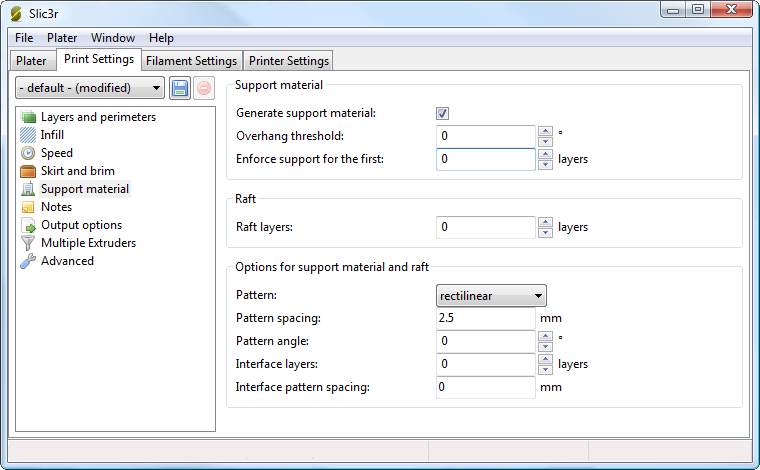
\includegraphics[keepaspectratio=true,width=1\textwidth]{expertmode/support/advanced_support.png}
\caption{Support structure options.}
\label{fig:advanced_support}
\end{figure}
\index{Print Settings!Support material!Generate support material}
\index{Print Settings!Support material!Overhang threshold}
\index{Print Settings!Support material!Enforce support}

The first thing to do is activate the support material option by checking the \texttt{Generate support material} box.  Providing a value of zero to the \texttt{Overhang threshold} parameter tells Slic3r to detect places to provide support automatically, otherwise the degrees given will be used.  Support generation is a relatively complex topic, and there are several aspects which determine the optimal support, it is strongly recommended to set the threshold to zero and allow Slic3r to determine the support required.

Small models, and those with small footprints, can sometimes break or detach from the bed.  Therefore the \texttt{Enforce support} option will cause support structures to be printed for the given number of layers, regardless of the angle threshold value.

To demonstrate the infill patterns the minimug model was tilted by 45° along the x axis, as shown in figure \ref{fig:support_minimug_45deg}.
\index{Print Settings!Support material!Pattern}

\begin{figure}[H]
\centering
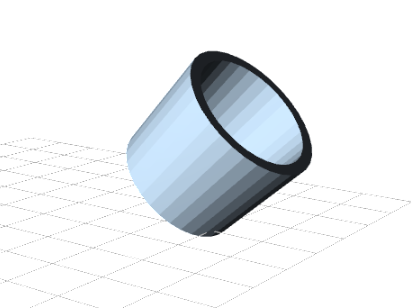
\includegraphics[keepaspectratio=true,width=0.75\textwidth]{expertmode/support/support_minimug_45deg.png}
\caption{Minimug model, tilted 45°.}
\label{fig:support_minimug_45deg}
\end{figure}

As with infill, there are several patterns available for the support structure.

\begin{figure}[H]
\centering
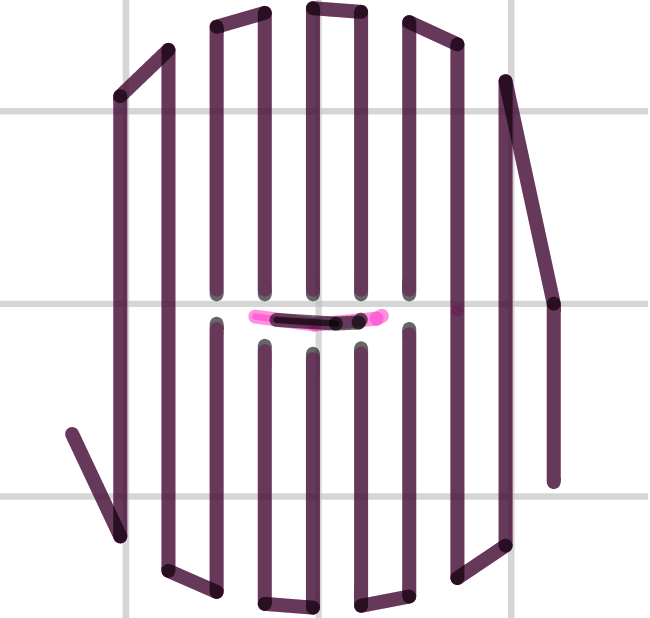
\includegraphics[keepaspectratio=true,width=0.2\textwidth]{expertmode/support/support_pattern_rectlinear.png}
\caption{Support infill pattern: Rectilinear}
\label{fig:support_pattern_rectlinear}
\end{figure}

\begin{figure}[H]
\centering
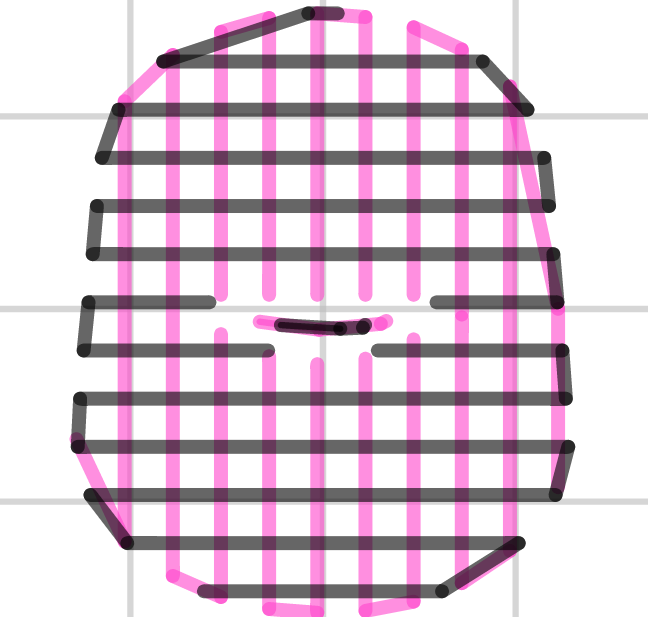
\includegraphics[keepaspectratio=true,width=0.2\textwidth]{expertmode/support/support_pattern_rectlinear_grid.png}
\caption{Support infill pattern: Rectilinear Grid}
\label{fig:support_pattern_rectlinear_grid}
\end{figure}

\begin{figure}[H]
\centering
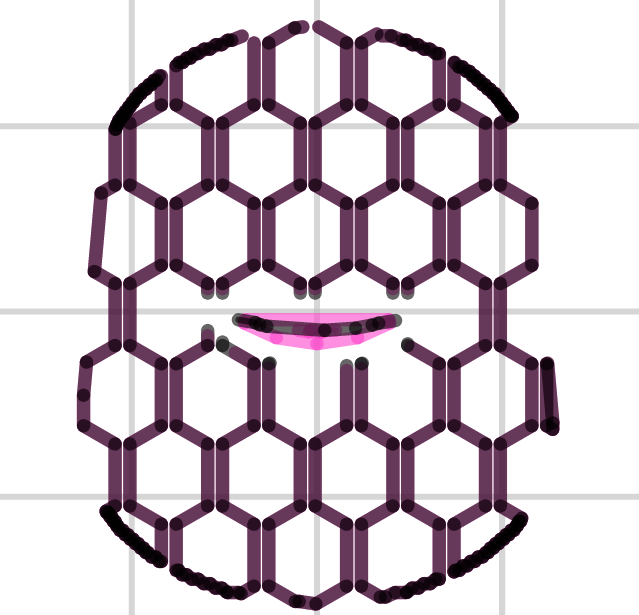
\includegraphics[keepaspectratio=true,width=0.2\textwidth]{expertmode/support/support_pattern_honeycomb.png}
\caption{Support infill pattern: Honeycomb}
\label{fig:support_pattern_honeycomb}
\end{figure}
\index{Print Settings!Support material!Pattern Spacing}
\index{Print Settings!Support material!Pattern Angle}

\texttt{Pattern Spacing} determines the distance between support lines, and is akin to infill density apart from being defined only in mm.  If changing this attribute take into account the width of the support extrusion and the amount of support material that will adhere to the object.

Care should be taken to choose a support pattern which matches the model, where the support material attaches perpendicularly to the wall of the object, rather than in parallel, so it will be easy to remove.  If the support structure does run along the length of a wall then the \texttt{Pattern Angle} option allows the direction of the support lines to be rotated.

\begin{figure}[H]
\centering
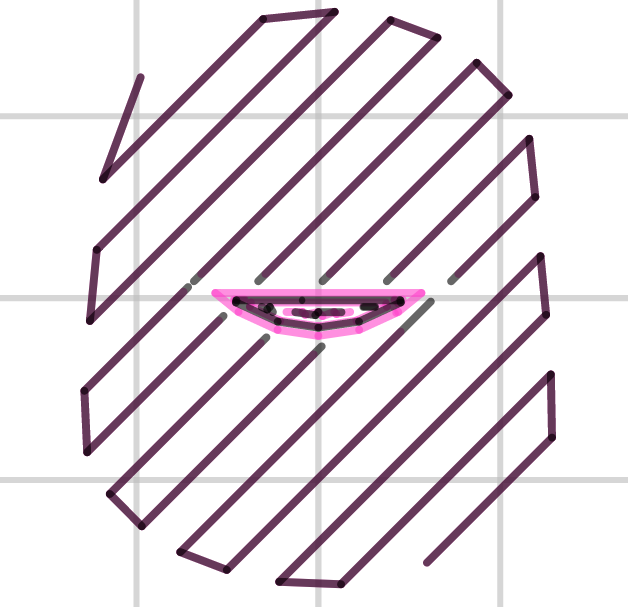
\includegraphics[keepaspectratio=true,width=0.2\textwidth]{expertmode/support/support_pattern_rectlinear_rotated.png}
\caption{Example of pattern angle rotated 45°.}
\label{fig:support_pattern_rectlinear_rotated}
\end{figure}


%TODO: Interface layers.


% section support (end)

\newpage

%!TEX root = Slic3r-Manual.tex

\section{Multiple Extruders} % (fold)
\label{sec:multiple_extruders}
\index{extruders!multiple}

A printer with more than one extruder can be used in different ways: The additional extruder could print a different colour or material; or it could be assigned to print particular features, such as infill, support or perimeters.  

Multi-material printing requires a suitably designed object usually written in AMF format as this can handle multiple materials (see Model Formats in §\ref{sub:model_formats}).  Details on how to create such a file are given below.


\subsection{Configuring Extruders} % (fold)
\label{sub:configuring_extruders}

In the \texttt{Printer Settings} tab there is an \texttt{Extruders} option, under \texttt{Capabilities}, which allows the number of extruders to be defined.  Incrementing this value will dynamically add another extruder definition to the left-hand pane.

\begin{figure}[H]
\centering
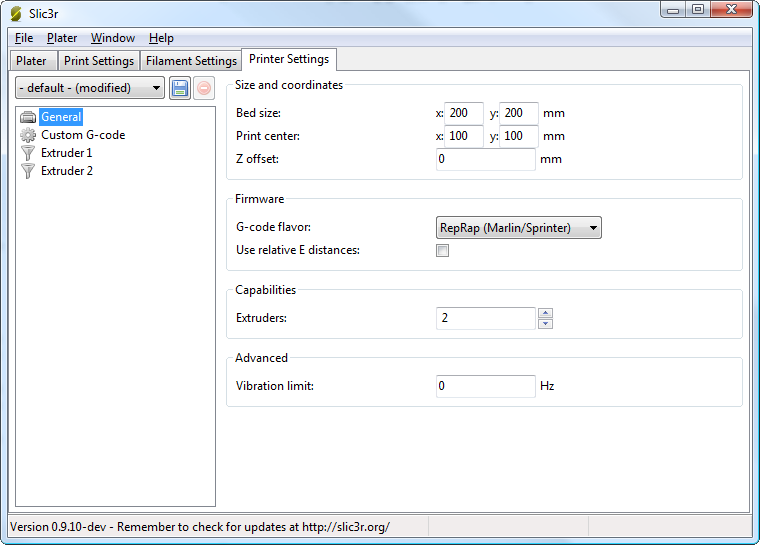
\includegraphics[keepaspectratio=true,width=0.75\textwidth]{expertmode/multipleextruders/printer_settings_general_multiple_extruder_options.png}
\caption{Multiple extruder options - Printer Settings Tab (General).  Note the two extruders defined in the left-hand pane.}
\label{fig:printer_settings_general_multiple_extruder_options}
\end{figure}

Each extruder can be configured as usual, however there are additional settings which must be set which are particular to multi-extruder setups.  

\begin{figure}[H]
\centering
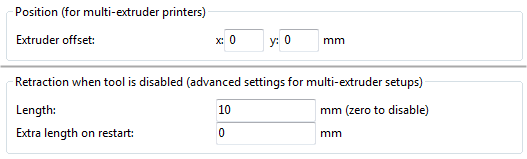
\includegraphics[keepaspectratio=true,width=0.75\textwidth]{expertmode/multipleextruders/printer_settings_extruder_multiple_extruder_options.png}
\caption{Multiple extruder options - Printer Settings Tab (Extruder).}
\label{fig:printer_settings_extruder_multiple_extruder_options}
\end{figure}

The \texttt{Extruder offset} is to be used should the firmware not handle the displacement of each additional nozzle.  Your firmware documentation should tell you if this is the case.  Each additional extruder is given an offset in relation to the first one.  If the firmware does handle this then all offsets can remain at 0,0.

Because the secondary extruder will be dormant whilst the first is working, and vice-versa, it is important that the material is sufficiently retracted to stop oozing.  As with the regular retraction settings (see p. \pageref{fig:retraction_settings}) the \texttt{Length} options is measured from the raw filament entering the extruder.

% subsection configuring_extruders (end)

\subsection{Assigning Filaments} % (fold)
\label{sub:assigning_filaments}

When a printer profile with multiple extruders has been selected the \texttt{Plater} tab allows the selection of a different filament for each extruder. 

\begin{figure}[H]
\centering
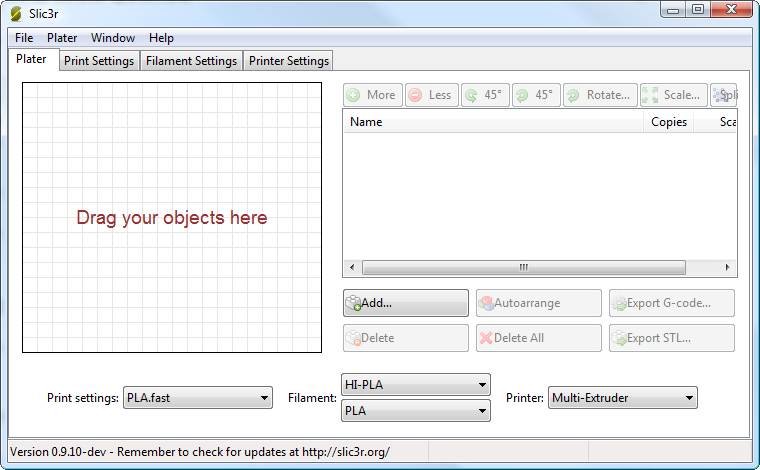
\includegraphics[keepaspectratio=true,width=0.75\textwidth]{expertmode/multipleextruders/plater_multi_filament.png}
\caption{Plater with multiple filament options.}
\label{fig:plater_multi_filament}
\end{figure}

% subsection assigning_filaments (end)

\subsection{Assigning Extruders for Single-material Objects} % (fold)
\label{sub:assigning_extruders}

For single material prints, where the secondary extruder is to be tasked with a particular extrusion, the \texttt{Multiple Extruders} section of the \texttt{Print Settings} tab gives the ability to assign an extruder to each extrusion type.

\begin{figure}[H]
\centering
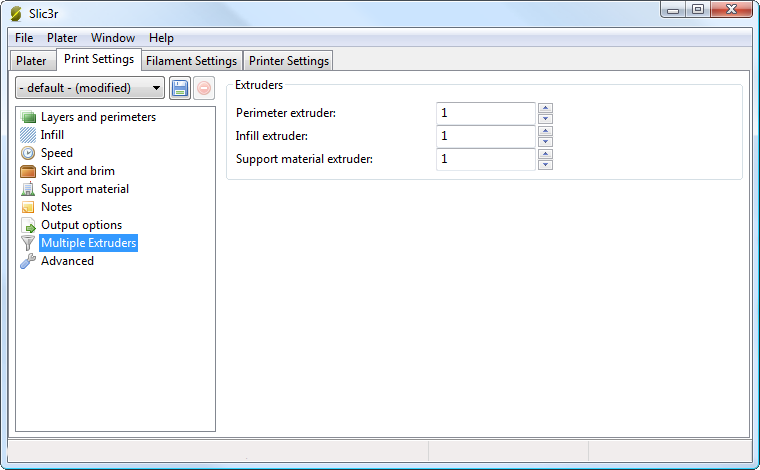
\includegraphics[keepaspectratio=true,width=0.75\textwidth]{expertmode/multipleextruders/print_settings_multiple_extruder_options.png}
\caption{Multiple extruder options - Print Settings Tab.}
\label{fig:advanced_multiple_extruder_options}
\end{figure}

% subsection assigning_extruders (end)

\subsection{Configuring Tool Changes} % (fold)
\label{sub:configuring_tool_changes}

The \texttt{Custom G-code} section of the \texttt{Printer Settings} tab has an option for inserting G-code between tool changes.  As with all custom G-code sections, placeholder variables can be used to reference Slic3r settings.  This includes the [previous\_extruder] and [next\_extruder] variables.

\begin{figure}[H]
\centering
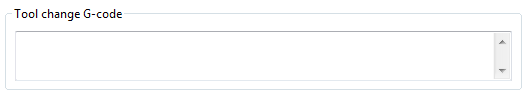
\includegraphics[keepaspectratio=true,width=0.75\textwidth]{expertmode/multipleextruders/printer_settings_custom_gcode.png}
\caption{Multiple extruder options - Tool change G-code.}
\label{fig:printer_settings_custom_gcode}
\end{figure}

% subsection configuring_tool_changes (end)


\subsection{Printing Multi-material Objects} % (fold)
\label{sub:printing_multi_material_objects}

If a multi-material AMF file already exists, because the CAD program can export such a format, then this can be loaded into Slic3r in the usual way.  The mapping between object materials and extruders is sequential, i.e. the first material is assigned to the first extruder, etc.

% subsection printing_multi_material_objects (end)


\subsection{Generating multi-material AMF files} % (fold)
\label{sub:generating_multi_material_amf_files}

Slic3r has the feature to combine multiple STL files into a multi-material AMF file.

\begin{itemize}
    \item Split the original design into the separate parts within the CAD program, and export each part as STL.
    \item Within Slic3r, choose \texttt{Combine multi-material STL files...} from the \texttt{File} menu.
    \item When prompted with a file dialog, choose the first STL, which will be assigned the first material (and hence the first extruder). Click \texttt{Open} to be prompted for the next STL, and so on until each STL is assigned a material.  To signal there are no more STL files, choose \texttt{Cancel}.
    \item The following file dialog prompts for the location and name of the AMF file.
\end{itemize}

Once generated the file can be loaded and printed as described above.

% subsection generating_multi_material_amf_files (end)

% section multipe_extruders (end)

\newpage

%!TEX root = Slic3r-Manual.tex

\section{Sequential Printing} % (fold)
\label{sec:sequential_printing}

\begin{figure}[H]
\centering
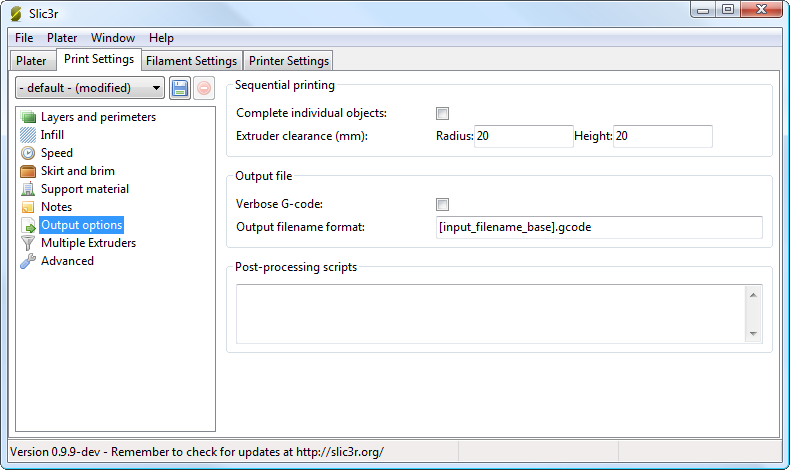
\includegraphics[keepaspectratio=true,width=0.75\textwidth]{expertmode/advanced_sequential_printing_options.png}
\caption{Sequential printing options.}
\label{fig:advanced_sequential_printing_options}
\end{figure}


% section sequential_printing (end)

\newpage

%!TEX root = Slic3r-Manual.tex

\section{Extrusion Width} % (fold)
\label{sec:extrusion_width}

\begin{figure}[H]
\centering
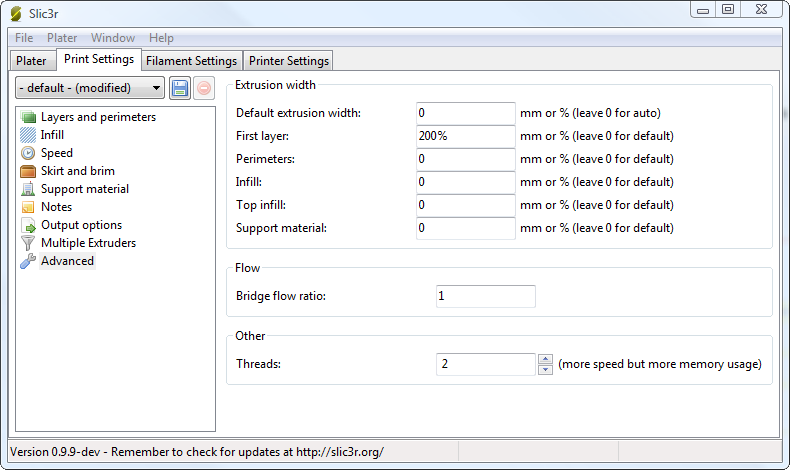
\includegraphics[keepaspectratio=true,width=0.75\textwidth]{expertmode/advanced_extrusion_widths_options.png}
\caption{Extrusion widths options.}
\label{fig:advanced_extrusion_widths_options}
\end{figure}


% section extrusion_width (end)
}
\fi
%%% END EXPERT MODE %%%

%%% CONFIGURATION ORGANIZATION %%%
\ifadvanced
\chapter{\emph{Configuration Organization}}
\thispagestyle{empty}
\markboth{Configuration Organization}{Slic3r User Manual}
{%!TEX root = Slic3r-Manual.tex

There are two ways in which to organise the configuration settings: exporting and importing the configuration settings, and profiles.  The former is available in both simple and expert mode, whereas profiles is only available in expert mode.

\section{Exporting and Importing Configuration} % (fold)
\label{sub:exporting_and_importing_configuration}
\index{configuration!export}
\index{configuration!import}

The current set of configuration options can be simply exported via the \texttt{Export Config} File menu option. This saves all the values into a text file with a \texttt{.ini} extension.  Previously saved files can be loaded with the \texttt{Load Config} menu option.

This gives a rudimentary means to store different configuration settings for different needs.  For example a set with slightly faster print speeds, or a different infill pattern.  However this way of organising things will quickly become frustrating, as each minor change to a parameter may have to be duplicated across many configurations.  For this reason, profiles are a more suitable way of managing multiple configurations.

This method also allows configuration to be transferred between machines, or stored remotely.

% section exporting_and_importing_configuration (end)


\section{Profiles} % (fold)
\label{sec:profiles}
\index{profiles}

After a few prints it will become apparent that it is worth having a set of configuration options to choose from, and that some parameters change at different rates as others.  In expert mode, profiles can be created for Print, Filament and Printer settings, with the expectation that the printer settings change least often, filament rarely, and the print settings could be changed for each model.  These different profiles can be mixed and matched as desired, and can be selected either in their respective tabs, or directly from the plater.

\subsection{Creating Profiles} % (fold)
\label{sub:creating_profiles}
\index{profiles!create}

Open the desired tab and change the settings as necessary.  Once satisfied, click the save icon to the left above the setting titles, and give a suitable name when prompted.

\begin{figure}[H]
\centering
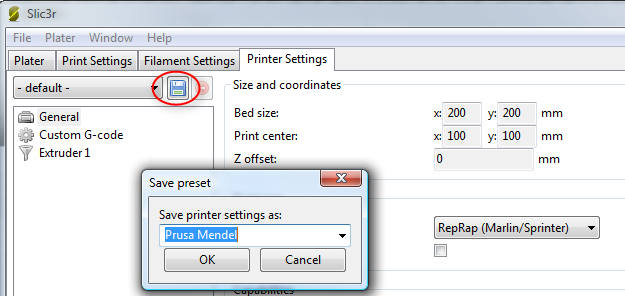
\includegraphics[keepaspectratio=true,width=0.75\textwidth]{organising/creating_a_profile.png}
\caption{Saving a profile.}
\label{fig:creating_a_profile}
\end{figure}

\index{profiles!delete}
Profiles can be deleted by choosing the profile to delete and clicking the red delete button next to the save button.

\begin{figure}[H]
\centering
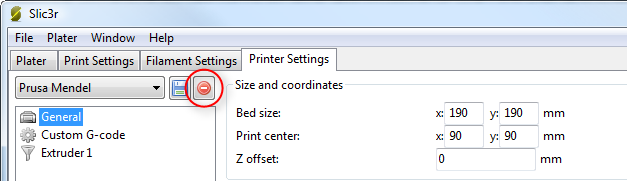
\includegraphics[keepaspectratio=true,width=0.75\textwidth]{organising/deleting_a_profile.png}
\caption{Deleting a profile.}
\label{fig:deleting_a_profile}
\end{figure}

% subsection creating_profiles (end)


% section profiles (end)}
\fi
%%% END CONFIGURATION ORGANIZATION %%%

%%% ADVANCED %%%
\ifadvanced
\chapter{\emph{Advanced Topics}}
\thispagestyle{empty}
\markboth{Advanced Topics}{Slic3r User Manual}
{%!TEX root = Slic3r-Manual.tex

%!TEX root = Slic3r-Manual.tex

\section{SVG Output} % (fold)
\label{sec:svg_output}
\index{SVG}
\index{DLP resin printer}
\index{powder-bed printer}

Slic3r can produce output for other types of 3D printers which require each layer to be represented as image, for example DLP resin or powder-bed printers.  These expect an image usually consisting of a white silhouette on a black background (See fig \ref{fig:example_svg_slice}).  Almost all image formats can be used (bmp, png, etc.), however, because the image may have to be scaled, it is usually desirable to use a vector format, rather than a bitmap format.  For this reason it is common to use Scalable Vector Graphics (SVG) format.

\begin{figure}[H]
\centering
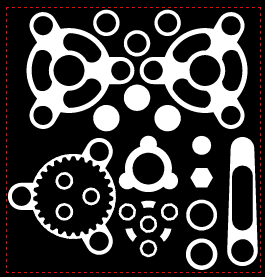
\includegraphics[keepaspectratio=true,width=0.5\textwidth]{advanced/svg_output/example_svg_slice.png}
\caption{Example SVG slice.}
\label{fig:example_svg_slice}
\end{figure}

\index{Menu!Slice to SVG...}

Slic3r provides the ability to produce SVG output suitable for such printers.  Instead of using the \texttt{Plater}, the process begins by selecting the \texttt{Slice to SVG...} option from the \texttt{File} menu.  This prompts for the source file (STL, OBJ or AMF), and when selected will prompt for where the output SVG file should be saved.  Slic3r will then go and produce the SVG file.

Attempting to view the SVG file in a browser will result in only the first layer being shown, and only the negative islands within the model (as the browser background is usually white).

\begin{figure}[H]
\centering
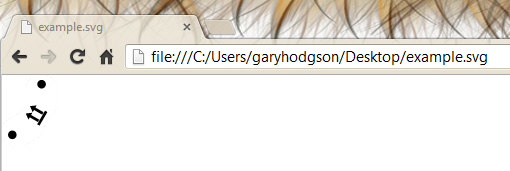
\includegraphics[keepaspectratio=true,width=0.75\textwidth]{advanced/svg_output/svg_direct_browser.png}
\caption{SVG in the browser.}
\label{fig:svg_direct_browser}
\end{figure}

For this reason a small web application was written to allow each slice to be displayed, and for it to be shown on a black background\footnote{\url{http://garyhodgson.github.io/slic3rsvgviewer}}.  Navigate to the application and drag and drop the SVG file onto the screen to have it load and display.

\begin{figure}[H]
\centering
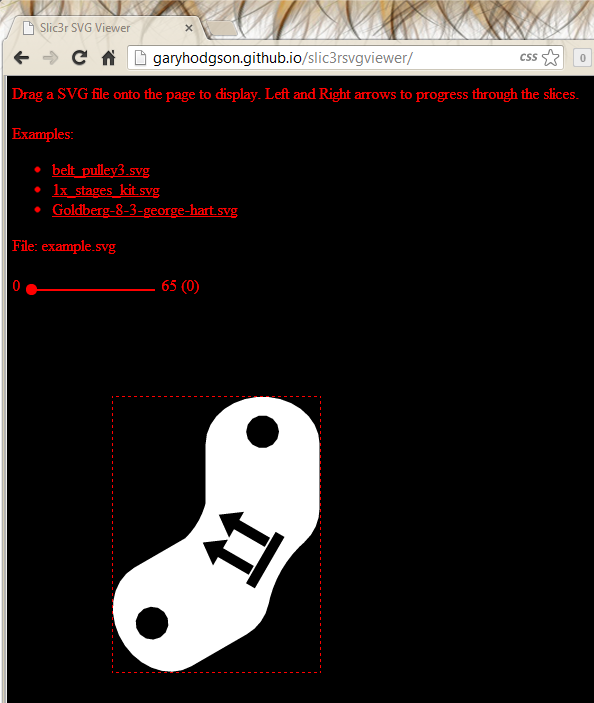
\includegraphics[keepaspectratio=true,width=0.75\textwidth]{advanced/svg_output/svg_slic3rsvg_viewer.png}
\caption{Slic3r SVG Viewer.}
\label{fig:svg_slic3rsvg_viewer}
\end{figure}

\subsection{SVG Settings} % (fold)
\label{sub:svg_settings}

The majority of options in Slic3r are not required when generating SVG, however the \texttt{Layer height} setting will dictate the number of layers.  Note that Slic3r restricts the layer height to be smaller than the nozzle diameter, so this may also have to increased if higher layers are desired.

% subsection svg_settings (end)

\subsection{Printing with SVG} % (fold)
\label{sub:printing_with_svg}

Whilst SVG output can be used in a range of printers, the following example shows how the file can be used with a DLP resin printer.  Using a modified version of Kliment's Printrun\footnote{\url{http://garyhodgson.com/reprap/projectlayer}} the SVG file can be loaded directly and sent to a DLP projector.  The Z axis is controlled via G-Code commands sent through the printcore component, which means that standard RepRap electronics, such as RAMPS, can be used.


\begin{figure}[H]
\centering
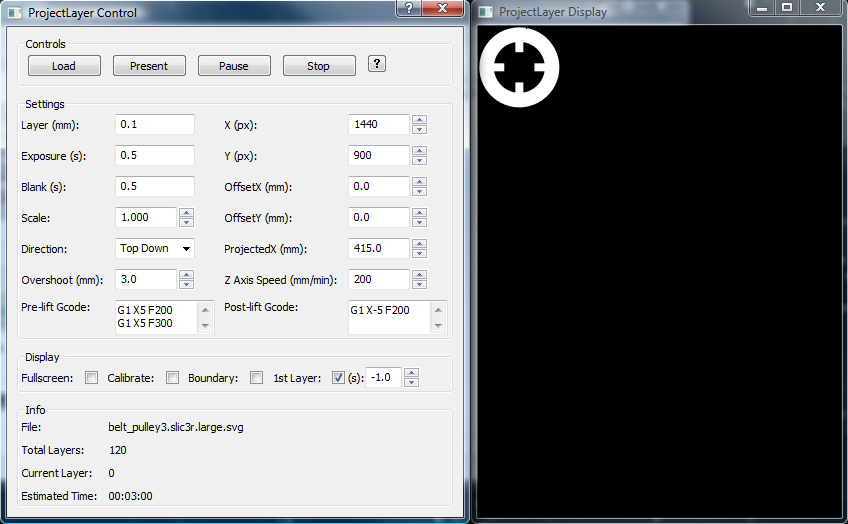
\includegraphics[keepaspectratio=true,width=0.75\textwidth]{advanced/svg_output/projectlayer.png}
\caption{Printing SVG with Projectlayer.}
\label{fig:projectlayer}
\end{figure}


% subsection printing_with_svg (end)

% section svg_output (end)

\newpage

%!TEX root = Slic3r-Manual.tex

\section{Command Line Usage} % (fold)
\label{sec:command_line_usage}

% section command_line_usage (end)

\newpage

%!TEX root = Slic3r-Manual.tex

\section{Post-Processing Scripts} % (fold)
\label{sec:post_processing_scripts}
\index{scripts}
\index{post processing}

There may be times when the G-Code generated by Slic3r has to be tweaked or modified after it has been created.  For this reason there exists the ability to run arbitrary scripts as part of the final steps in the slicing process\footnote{\url{https://github.com/alexrj/Slic3r/wiki/Writing-post-processing-scripts}}.

In the \texttt{Output options} section of the \texttt{Print Settings} tab lies the \texttt{Post-processing scripts} option.  The absolute path to each script can be added, separated by semicolons. Each scripts should be recognised by the host system, and be executable.

\begin{figure}[H]
\centering
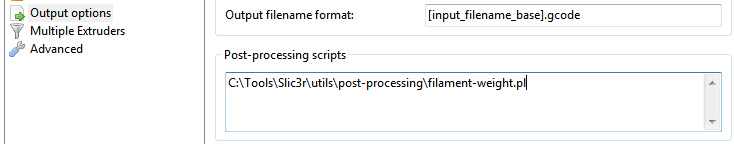
\includegraphics[keepaspectratio=true,width=1\textwidth]{advanced/post_processing_scripts/post_processing_scripts_options.png}
\caption{Post-processing script option.}
\label{fig:post_processing_scripts_options}
\end{figure}

Each script will be passed the absolute path of the G-Code file that Slic3r generates.  All Slic3r configuration options are made available to the scripts by way of environment variables.  These all begin with \texttt{SLIC3R\_}.  The following script would write out all Slic3r options to standard output:

\begin{figure}[H]
\small
\begin{verbatim}
        #!/bin/sh
        echo "Post-processing G-code file: $*"
        env | grep ^SLIC3R
\end{verbatim}
\caption{Example post-processing script to display Slic3r environment variables.}
\label{fig:exaple_post_processing_script_env_vars}
\end{figure}

Example scripts can be found in the GitHub repository\footnote{\url{https://github.com/alexrj/Slic3r/tree/master/utils/post-processing}}.


Perl's in-place mode (\texttt{perl -i}) makes it easy to modify the contents of the G-Code file, without having to copy, edit, then replace the original.  The following example will simply output the contents to standard output:

\begin{figure}[H]
\small
\begin{verbatim}
        #!/usr/bin/perl -i
        use strict;
        use warnings;

        while (<>) {
             # modify $_ here before printing
             print;
        }
\end{verbatim}
\caption{Example post-processing script to print each line to output.}
\label{fig:exaple_post_processing_script_print_lines}
\end{figure}



% section post_processing_scripts (end)

\newpage}
\fi
%%% END ADVANCED %%%

%%% TROUBLESHOOTING %%%
\ifadvanced
\chapter{\emph{Troubleshooting}}
\thispagestyle{empty}
\markboth{Troubleshooting}{Slic3r User Manual}
{%!TEX root = Slic3r-Manual.tex

%!TEX root = Slic3r-Manual.tex

\section{Z Wobble} % (fold)
\label{sec:z_wobble}
\index{Z Wobble}


Undulations in the walls of a print may be due to wobble in the Z axis.  A thorough analysis of the potential causes is given by whosawhatsis\footnote{\url{http://goo.gl/iOYoK}} in his article "Taxonomy of Z axis artifacts in extrusion-based 3d printing"\footnote{\url{http://goo.gl/ci9Gz}}, however one point of particular interest for users of Slic3r is the wobble caused by motor steps not matching the pitch of the Z rods thread.  This can be addressed by ensuring the \texttt{Layer Height} setting is a multiple of the full step length.


The relevant part of the above paper is quoted here:

\quote{To avoid Z ribbing, you should always choose a layer height that is a multiple of your full-step length. To calculate the full-step length for the screws you're using, take the pitch of your screws (I recommend M6, with a pitch of 1mm) and divide by the number of full-steps per rotation on your motors (usually 200). Microsteps are not reliably accurate enough, so ignore them for this calculation (though using microstepping will still make them smoother and quieter). For my recommended M6 screws, this comes out to 5 microns. It's 4 microns for the M5 screws used by the i3, and 6.25 microns for the M8 screws used by most other repraps. A layer height of 200 microns (.2mm), for example, will work with any of these because 200 = 6.25 * 32 = 5 * 40 = 4 * 50.}


% section z_wobble (end)

\newpage

}
\fi
%%% END TROUBLESHOOTING %%%

%%% SUPPORT %%%
\ifsupport
\chapter{\emph{Slic3r Support}}
\thispagestyle{empty}
\markboth{Slic3r Support}{Slic3r User Manual}
{%!TEX root = Slic3r-Manual.tex
\section{Slic3r Support} % (fold)
\label{sec:slic3r_support}

\index{community support}
\index{Freenode}
\index{IRC}
\index{RepRap}
\index{forums}
\index{website}
\index{blog}

A variety of resources are available to provide support for Slic3r.
\subsection{Wiki and FAQ} % (fold)
\label{sub:wiki_and_faq}
The wiki provides up-to-date documentation, and a FAQ section which may help resolve any queries or issues.
\begin{itemize}
    \item \url{https://github.com/alexrj/Slic3r/wiki/Documentation}
    \item \url{https://github.com/alexrj/Slic3r/wiki/FAQ}
\end{itemize}
% subsection wiki_and_faq (end)

\subsection{Blog} % (fold)
\label{sub:blog}
Tips, hints and advice are published on the Slic3r blog.
\begin{itemize}
    \item \url{http://slic3r.org/blog}
\end{itemize}
% subsection blog (end)

\subsection{IRC} % (fold)
\label{sub:irc}

Found on the \texttt{irc.freenode.net} server, the following chat rooms are often filled with people who can provide real-time help:
\begin{itemize}
\item \texttt{\#reprap}: Highly active community of the RepRap project with many users of Slic3r.
\item \texttt{\#slic3r}: Slic3r chat room where Slic3r developers and users can give help.
\end{itemize}

% subsection irc (end)

\subsection{RepRap.org Forum} % (fold)
\label{sub:reprap_org_forum}


A dedicated forum for Slic3r exists in the RepRap forums.
\begin{itemize}
    \item \url{forums.reprap.org/list.php?263}
\end{itemize}

% subsection reprap_org_forum (end)

\subsection{Issue Tracker} % (fold)
\label{sub:issue_tracker}

If a bug may have been found in the software then an issue may be raised in the project issue tracker.

\begin{itemize}
    \item \url{github.com/alexrj/Slic3r/issues}
\end{itemize}

\textbf{Please} take the time to read through the existing issues to see whether the problem has already been submitted.  Also make sure that the problem is a bug in the application, support related questions should not be submitted.

If the bug appears to be unreported then please read the bug report guide before submitting: \url{http://git.io/11Hy\char`_w}.

% subsection issue_tracker (end)

% section slic3r_support (end)
}
\fi
%%% END SUPPORT %%%

%%% END MAINMATTER %%%
%%% BEGIN BACKMATTER %%%
\backmatter

% section section_name (end)

%%% INDEX %%%
\clearpage
\printindex
%%% END INDEX %%%

%%% GLOSSARY %%%
% Presently disabled, until filled
% Sample:
%\glossary{glossary}{A list of terms and their descriptions.}
%\clearpage
%\printglossary
%%% END GLOSSARY %%%

%%% COLOPHON %%%
\ifcolophon
%%% skip a couple pages
\pagebreak{}
\thispagestyle{empty}
\begingroup 
\vfill\null 
\endgroup
\pagebreak{}
\thispagestyle{empty}
{%%% COLOPHON %%%
\begin{vplace}
\centering
\emph{\LARGE Colophon}

\rule{0.5\textwidth}{0.4pt}\\[\baselineskip]

{\tiny Created with 100\% Free/Libre Software}

GNU/Linux

{\LaTeX} Memoir

% XXX surely a less dumb way to make some space :)
\rule{0\textwidth}{0pt}\\[\baselineskip]%
\rule{0.5\textwidth}{0.4pt}\\[\baselineskip]
\end{vplace}
%%% END COLOPHON %%%
}
\fi
%%% END COLOPHON %%%
%%% END BACKMATTER %%%


\end{document}

